\documentclass[12pt,a4paper]{scrartcl}

%%%%%
% Header for solutions for the course Machine Learning for Computer Vision
% Summer 2017
%%%%%

\usepackage[utf8]{inputenc}
\usepackage[english]{babel}

\usepackage{
  amsmath,
  graphicx,
  tabularx,
  caption,
  subcaption,
  float,
  listingsutf8,
}

\usepackage[load-configurations = abbreviations]{siunitx}
\usepackage{hyperref}
\usepackage[english]{cleveref}

%%%%% format settings
%------------
% \setlength{\parindent}{0pt} %no indent
%------------

%%%%% settings for listings
\lstset{
  language=python,
  basicstyle=\footnotesize,  % font size
  showspaces=false,
  showstringspaces=false,
  frame=single, %tb
  breaklines=true,
  % backgroundcolor=\color[RGB]{245,245,244},
  % otherkeywords={self},             % Add keywords here
  % keywordstyle=\color{blue},
  % commentstyle=\it\color[RGB]{0,96,96}\ttfamily,
  % stringstyle=\color[RGB]{255,140,0},
  % numbers=left,
  % stepnumber=5,
}

%%% commands
%------------
\newcommand{\code}{\texttt}
%------------

% \usepackage[dvipdfmx]{graphicx}


\author{Kodai Matsuoke, Yuyan Li}
\subject{Machine Learning for Computer Vision}
\title{Exercise 6}
% \subtitle{}
\date{June 2}


\begin{document}

\maketitle

\section{Potts MRF with chain structure}

We implemented a function which finds a argmin of Potts MRF with chain structure. The code is in Listing \ref{lst:chain}.

\lstinputlisting[caption=Solver of Potts MRF with chain structure,linerange={15-34},label=lst:chain]{Exercise6.py}

The result for different betas is in Fig \ref{fig:result1}
We can see from the result that the bigger the beta is, the more pixels are in the same state.

\begin{figure}
	\centering
    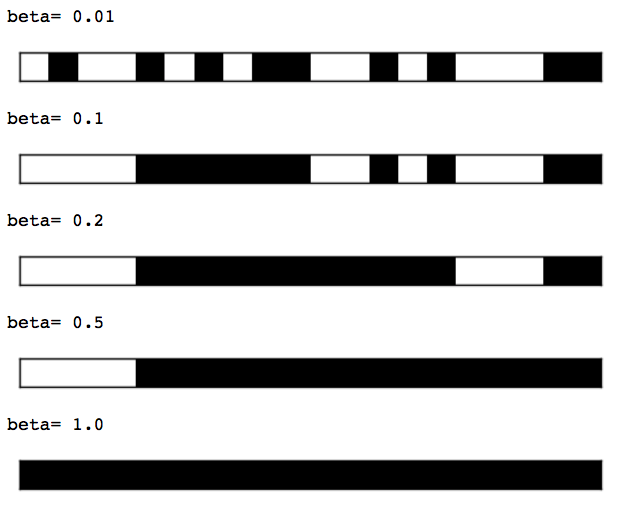
\includegraphics[width=15cm]{result1.png}
\end{figure}

When unary energies are [-1,1], we cannot use Dijkstra Alogorithm. Istead, we can use Bellman-Ford alpgorithm with which we are able to handle negative weights. The other solution for this problem is to set the offset so that all the weights are positive. Since adding scalar to every unary elements does not change the structure, energies between [-1,1] is identical to [0,2].


\section{Potts MRF with grid structure}
\subsection{Implementation}
Code to optimize \(E_{h}(X)\) and \(E_{v}(X)\) is in Listing 2.
\lstinputlisting[caption=Solver of Potts MRF with grid structure,linerange={36-52},label=lst:grid]{Exercise6.py}

The result for different betas is shown below.
The bigger the beta is, the more pixels (either in horizontal or vertical direction) are in the same state.

\begin{figure}
	\centering
    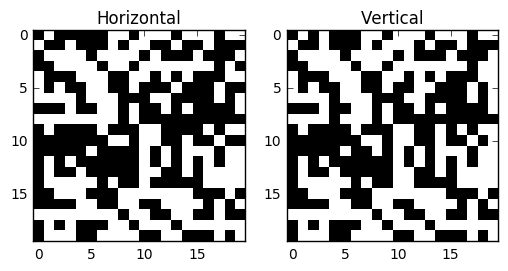
\includegraphics[width=9cm]{result2.png}

    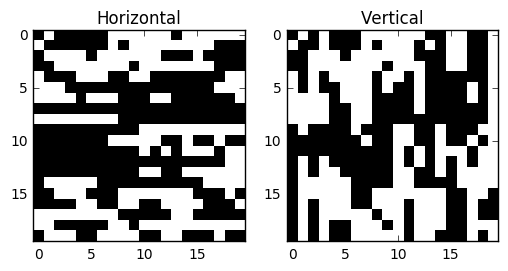
\includegraphics[width=9cm]{result3.png}

    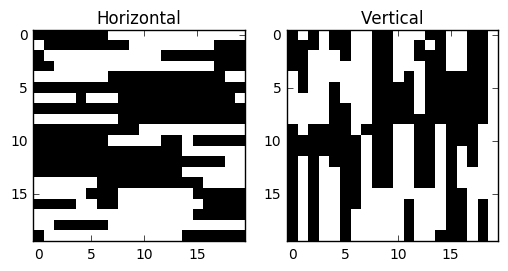
\includegraphics[width=9cm]{result4.png}

    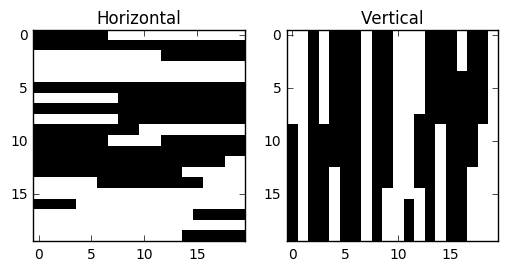
\includegraphics[width=9cm]{result5.png}

    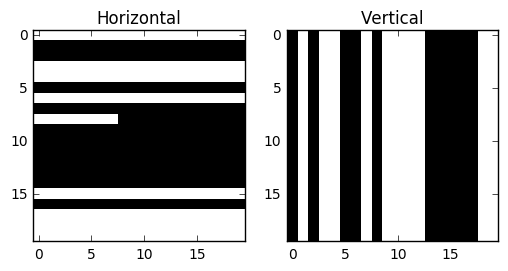
\includegraphics[width=9cm]{result6.png}
\end{figure}

\subsection{Interpretation}
By definition of \(E_{h}\) and \(E_{v}\),
\[
E_{h}(\hat{X}) \geq E_{h}(\hat{X}^h)
\quad and \quad 
E_{v}(\hat{X}) \geq E_{v}(\hat{X}^v)
\]
are always satisfied. So, 
\[
E(\hat{X}) = E_{h}(\hat{X}) + E_{v}(\hat{X}) \geq E_{h}(\hat{X}^h) + E_{v}(\hat{X}^v)
\]
is concluded.


When \(\hat{X}^h = \hat{X}^v = \hat{X}^{hv}\)
\[
\forall X, E(X)=E_{h}(X)+E_{v}(X) \geq E_{h}(\hat{X}^h) + E_{v}(\hat{X}^v)=E(\hat{X}^{hv})
\]
This indicates
\[
\hat{X}^{hv} = \hat{X}
\]

% \lstinputlisting[language=LANG,caption=CAPTION,label=lst:LABEL]{PATH/TO/CODE.file}

\end{document}